\documentclass[runningheads,envcountsame,orivec]{llncs}
\usepackage[T1]{fontenc}
\usepackage[utf8]{inputenc}
\usepackage{lmodern}
\usepackage{microtype}
\usepackage{amsmath,amssymb,mathtools}
\usepackage{booktabs}
\usepackage{tikz}
\usepackage[hidelinks]{hyperref}
\urlstyle{same}

\newcommand{\E}{\mathbb E}
\newcommand{\PP}{\mathbb P}
\newcommand{\ind}{\mathbf 1}
\newcommand{\ch}{\operatorname{ch}}
\newcommand{\parnt}{\operatorname{par}}
\newcommand{\nil}{\bot}
\newcommand{\R}{\mathcal R}
\newcommand{\coef}[2]{[z^{#1}]#2}

\begin{document}
\title{Exact Matching in Growing Random Trees\texorpdfstring{\\}{ }with Constant Expected Update Cost}
\titlerunning{Exact Matching in Growing Random Trees}
\author{Marek Ga\l{}\k{a}zka}
\authorrunning{M. Ga\l{}\k{a}zka}
\institute{Faculty of Mathematics and Computer Science,\\
Adam Mickiewicz University, Pozna\'n, Poland}
\maketitle

\begin{abstract}
We analyze standard local maintenance of an explicit maximum matching in
growing trees. Under attachment with weight $1+\beta|\ch(v)|$,
$\beta\ge0$, the expected update time and recourse are constant, with
linear space and constant-time queries. A coefficientwise comparison
bounds expected weighted root sensitivity by one. We identify the
limiting update distribution throughout this family and prove that the
largest inspection count divided by $\log N/\log\log N$ converges
almost surely to one. Both results transfer to attachment proportional
to $\deg(v)+\delta$, $\delta>-1$, from a seed edge; ordinary
degree-proportional attachment has expected inspection count at most
$3/2$. For uniform attachment we additionally obtain the exact mean
$2-1/n$ and an $L^1$ bound $O(N^{-1/3}(\log N)^{2/3})$ for total
inspections normalized by $N$. Our contribution is the probabilistic
analysis of a known deterministic propagation scheme.
\keywords{Dynamic graph algorithms \and Maximum matching \and Preferential attachment \and Recourse \and Average-case analysis}
\end{abstract}

\section{Introduction}

A matching pairs vertices along edges, with no vertex used twice;
a maximum matching uses as many pairs as possible. On a static tree,
it is computed by a simple linear-time dynamic program. After adding
a leaf, however, its local states can change along a long path towards
the root (Fig.~\ref{fig:propagation}). How much work is needed over a
growing sequence of trees? We prove an exact expected cost below two
vertex inspections when each new leaf chooses its parent uniformly,
and constant expected cost throughout a family of preferential
attachment laws.

The local propagation scheme and the static binary recurrence are
known. Our contribution is their analysis under uniform recursive
growth: exact finite-size update identities, constant expected
recourse for an explicit optimum, the limiting update law, a
quantitative law of large numbers for cumulative inspections, and the
first-order maximum with leading constant one. Root sensitivity
drives the local results; an additive representation of the execution
history and long fringe paths yield the global ones. We then prove a
coefficientwise sensitivity bound for every affine attachment weight
$1+\beta\lvert\ch(v)\rvert$, $\beta\ge0$, and transfer it to
ordinary degree-based attachment. The extension gives constant expected
cost, a parameter-dependent limiting update law, and the same sharp
first-order maximum throughout the family.

\begin{figure}[t]
\centering
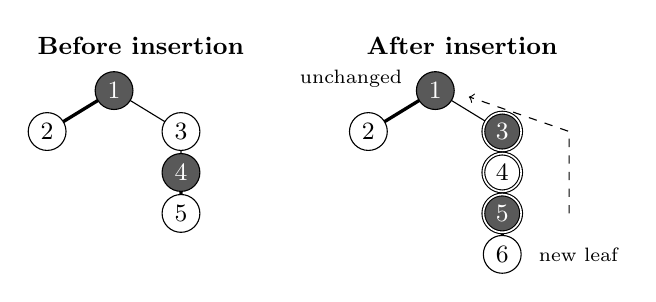
\begin{tikzpicture}[x=0.85cm,y=0.52cm,
 vertex/.style={circle,draw,minimum size=4.8mm,inner sep=0pt,font=\small},
 one/.style={vertex,fill=black!65,text=white},
 zero/.style={vertex,fill=white},
 changed/.style={double,double distance=0.6pt},
 match/.style={line width=1.2pt}]
 \begin{scope}
  \node[font=\small\bfseries] at (0.4,5.1) {Before insertion};
  \draw (0,4)--(-1,3) (0,4)--(1,3)--(1,2)--(1,1);
  \draw[match] (0,4)--(-1,3) (1,2)--(1,1);
  \node[one] at (0,4) {1}; \node[zero] at (-1,3) {2};
  \node[zero] at (1,3) {3}; \node[one] at (1,2) {4};
  \node[zero] at (1,1) {5};
 \end{scope}
 \begin{scope}[shift={(4.8,0)}]
  \node[font=\small\bfseries] at (0.4,5.1) {After insertion};
  \draw (0,4)--(-1,3) (0,4)--(1,3)--(1,2)--(1,1)--(1,0);
  \draw[match] (0,4)--(-1,3) (1,3)--(1,2) (1,1)--(1,0);
  \draw[->,dashed] (2,1)--(2,3)--(0.5,3.85);
  \node[one] at (0,4) {1}; \node[zero] at (-1,3) {2};
  \node[one,changed] at (1,3) {3};
  \node[zero,changed] at (1,2) {4};
  \node[one,changed] at (1,1) {5}; \node[zero] at (1,0) {6};
  \node[font=\scriptsize,anchor=east] at (-0.35,4.3) {unchanged};
  \node[font=\scriptsize,anchor=west] at (1.4,0) {new leaf};
 \end{scope}
\end{tikzpicture}
\caption{Adding leaf 6 flips states at 5, 4, and 3 (double circles).
The root 1 is inspected but stays in state one because leaf 2 has state
zero; hence $K_5=3$ and $U_5=4$. White and filled circles denote states
zero and one, respectively; thick edges form maximum matchings.
The dashed arrow traces the upward inspections. State zero does not
mean unmatched: vertex 2 is matched to the root in both trees.}
\label{fig:propagation}
\end{figure}

\paragraph{Related work.}
Janson~\cite{Janson2020} gives the classical binary recurrence and its
relation to independence number, maximum matching, and minimum vertex
cover. Fuchs et al.\ \cite{Fuchs2020} study static parameters of random
recursive trees. We use the general fringe-subtree identities and
covariance formulas of Holmgren and Janson~\cite{HolmgrenJanson2015},
including their version retaining arrival labels. Our analysis concerns
changes between successive trees and the resulting execution cost.
The preferential family is a standard increasing-tree model
\cite{SeelbachWagner2022}; Janson's static independence-number results
also cover preferential attachment, but do not analyze this update cost.

For arbitrary dynamically changing trees, Gupta and Sharma
\cite{GuptaSharma2009} maintain exact matching cardinality in
$O(\log n)$ update time using top trees. Tirodkar and Vishwanathan
\cite{TirodkarVishwanathan2018} give constant-time approximate matching
in incremental trees. Bosek et al.\ \cite{Bosek2018} bound the total
shortest augmenting-path length by $O(n\log n)$ for trees under
one-sided bipartite arrivals, a different model. Change propagation is
a standard dynamization method~\cite{Acar2004}; pivotal vertices also
arise in random tree automata~\cite{Johnson2020}. These are existing
tools and context, rather than claims of novelty here.

\section{Model and main result}\label{sec:model}

Let $T_1$ consist of the root $1$. For $n\ge1$, obtain $T_{n+1}$ by adding
vertex $n+1$ and the edge $\{P_{n+1},n+1\}$, where the variables
$P_{n+1}$ are independent and uniform on $\{1,\ldots,n\}$. Unless another law is explicitly specified, we use this uniform model;
Section~\ref{sec:preferential} defines the nonuniform laws.
The parent $P_{n+1}$ is supplied to the update algorithm. There are no deletions or
edge weights. We use a word-RAM in which vertex identifiers and counters
up to the current input size fit in a word.

For a rooted tree $T$, write $T_v$ for the subtree rooted at $v$ and
$\nu(T)$ for its maximum matching cardinality. Define
\begin{equation}\label{eq:state}
 d(v)=\ind\{\text{some }u\in\ch(v)\text{ has }d(u)=0\}.
\end{equation}
In particular, a leaf has state zero. After an insertion the algorithm
updates the parent of the new leaf, then proceeds to successive ancestors
while their states change. It stops at the first unchanged state or after
processing the root. Let $K_n$ be the number of \emph{old} vertices whose
states change in $T_n\to T_{n+1}$, and let $U_n$ be the number of old
vertices inspected by this upward propagation loop, including the final
unchanged one when present. It does not count the subsequent commit of
recorded matching-edge changes; that also takes $O(1+U_n)$ time.

\begin{theorem}\label{thm:main}
There is a deterministic algorithm maintaining a maximum matching $M_n$
of $T_n$ using $O(n)$ words of space and $O(1+U_n)$ time for the next
insertion. Cardinality, mate, and edge-membership queries take $O(1)$ time
after each completed insertion. For every $n\ge1$,
\begin{equation}\label{eq:mainmeans}
 \E K_n=1,\qquad \E U_n=2-\frac1n,
 \qquad \E\lvert M_{n+1}\triangle M_n\rvert\le3.
\end{equation}
Moreover,
\begin{equation}\label{eq:moment2main}
 \E 2^{K_n}=3-\frac1n,
 \qquad \sup_{n\ge1}\E m^{K_n}\le e\,m!
 \quad\text{for every integer }m\ge1.
\end{equation}
For every $a>0$ there is a constant $C_a$ such that, for all sufficiently
large $N$,
\begin{equation}\label{eq:seqbound}
 \PP\left(\max_{1\le n<N}U_n>
 C_a\frac{\log N}{\log\log N}\right)\le N^{-a}.
\end{equation}
\end{theorem}

The expected total number of old-vertex inspections in building $T_N$ is
exactly $2(N-1)-H_{N-1}$, where $H_j=\sum_{i=1}^j1/i$ and $H_0=0$.
Thus the total expected running time is linear. Expectations average
over the entire growth history, rather than conditioning on every
realized $T_n$. Extending a rooted path changes every old state; on
such a path, even averaging over the next parent gives
$\E[U_n\mid T_n]=\Theta(n)$: approximately half the sites propagate
to the root, with depths summing to $\Theta(n^2)$.

Sections~\ref{sec:limit}--\ref{sec:maximum} give the limiting update
law, cumulative cost, and longest propagation. The maximum result
concerns this algorithm, rather than all dynamic matching algorithms.

\section{The local algorithm}\label{sec:algorithm}

We first record the standard static invariant, including a convenient
representation of a matching. Its first part is the complement of the
essential-vertex recurrence in \cite{Janson2020}.

\begin{lemma}\label{lem:static}
For every rooted tree $T$,
\begin{equation}\label{eq:additive}
 \nu(T)=\sum_{v\in T}d(v).
\end{equation}
Choosing one zero-state child $c(v)$ for each vertex with $d(v)=1$
produces a maximum matching
$M=\{\{v,c(v)\}:d(v)=1\}$.
\end{lemma}
\begin{proof}
Let $\nu_0(T_v)$ denote the maximum matching cardinality when $v$ is
unmatched within $T_v$. Then
$\nu_0(T_v)=\sum_{u\in\ch(v)}\nu(T_u)$.
Writing $\delta(u)=\nu(T_u)-\nu_0(T_u)$, matching $v$ to a child $u$
improves this sum by $1-\delta(u)$. Induction from the leaves gives
$\delta(v)\in\{0,1\}$ and
$\delta(v)=1$ if and only if some child has $\delta(u)=0$. Hence
$\delta(v)=d(v)$, and summing the recurrence proves
\eqref{eq:additive}. The proposed matching edges are disjoint: their
parent endpoints have state one, their child endpoints have state zero,
and each child has only one parent. Their number is $\sum_vd(v)$.
\end{proof}

Store $d(v)$, its parent, a doubly linked list $L(v)$ of zero-state
children, and a selected child $c(v)$ when $d(v)=1$. Child list handles
give $O(1)$ insertions and deletions. Maintain $\mu=\sum_vd(v)$;
retain a valid selected child, otherwise choose the list head.

\begin{figure}[t]
\hrule\smallskip
\textbf{InsertLeaf($x,p$)} \quad (a new vertex $x$ with parent $p$)
\begin{enumerate}
\setlength{\itemsep}{1pt}
\item Set $\parnt(x)=p$, $d(x)=0$, $L(x)=\varnothing$, $c(x)=\nil$;
      insert $x$ into $L(p)$ and set $v=p$.
\item Set $b=d(v)$ and $d(v)=\ind\{L(v)\ne\varnothing\}$;
      update $\mu\gets\mu+d(v)-b$.
\item Record a new choice for $c(v)$: none if $d(v)=0$; otherwise retain
      the old choice if it is still in $L(v)$, or choose the list head.
\item If $d(v)=b$ or $v$ is the root, go to step 6.
\item Put $q=\parnt(v)$. Insert $v$ into $L(q)$ if $d(v)=0$, and remove
      it otherwise. Set $v=q$ and return to step 2.
\item Commit recorded choices: delete all obsolete matching edges,
      then add all new matching edges and store the new selected children.
\end{enumerate}
\smallskip\hrule
\caption{Each pass through steps 2--5 inspects one old vertex.}
\label{fig:algorithm}
\end{figure}

A selected child is tested in constant time using its current state.
Record witness replacements during propagation; deleting obsolete edges
before additions keeps the explicit edge set a matching throughout the
commit. Queries are issued between completed insertions.

\begin{lemma}\label{lem:implementation}
The algorithm is correct for every sequence of leaf insertions. An
insertion takes $O(1+U_n)$ time and changes at most $K_n+2$ matching
edges. Its space and query bounds are as in Theorem~\ref{thm:main}.
\end{lemma}
\begin{proof}
Only ancestors of the new leaf can change state. At an inspected vertex,
the children already have their new states, so its updated list gives
the correct value in \eqref{eq:state}. If that value is unchanged, the
parent receives the same input as before and no higher state can change.
Otherwise the list update at the parent is exactly the required one.
Thus all states and lists are correct upon termination. The global
counter and Lemma~\ref{lem:static} give the optimum cardinality and
matching.

Every pass performs a constant number of list, counter, and witness
operations. A changing state adds or deletes exactly one selected
downward edge. The final unchanged vertex may replace its selected
child, costing at most two further edge changes. There are no downward
edges at the new leaf. This proves the recourse bound; the number of
recorded changes and the commit time are also $O(1+U_n)$.

Each vertex requires a constant number of words. To answer a mate query
at $v$, return $c(v)$ when $d(v)=1$; otherwise return $\parnt(v)$ if
that parent selects $v$, and report unmatched otherwise. The cardinality
is $\mu$. For a parent--child edge, membership is tested by the parent's
selected-child pointer. Since labels increase down the tree, the smaller
endpoint is the only possible parent for an arbitrary queried pair.
\end{proof}

\section{Root sensitivity and the exact mean}\label{sec:mean}

For a rooted tree $T$, let $B(T)$ be the number of vertices at which
attaching a new leaf would change the root state. This counts insertion
locations, not changed vertices. If the root has $q$ zero-state children,
then
\begin{equation}\label{eq:Brec}
 B(T)=
 \begin{cases}
  1+\sum_{u\in\ch(r)}B(T_u),&q=0,\\
  B(T_{u_0}),&q=1,\ \text{with unique zero-state child }u_0,\\
  0,&q\ge2.
 \end{cases}
\end{equation}
Indeed, a direct attachment changes a zero-state root. A change inside
one child subtree affects the root precisely when all other children
have state one. Two zero-state children prevent any single attachment
from changing the root.

\begin{lemma}\label{lem:influence}
For a uniform recursive tree of every size $n\ge1$, $\E B(T_n)=1$.
\end{lemma}
\begin{proof}
Use exponential generating functions over increasing rooted trees on
the label set $\{1,\ldots,n\}$. There are $(n-1)!$ such trees, so their
generating function is
\[
 \R(z)=\sum_{n\ge1}\frac{z^n}{n}=-\log(1-z).
\]
Let $A_i(z)$ enumerate trees whose root has state $i$. Removing the
root, which has the smallest label, leaves a set of child trees. A
zero-state root has only one-state children. Consequently,
\begin{equation}\label{eq:A}
 A_0'=e^{A_1},\qquad A_0+A_1=\R,
 \qquad e^{A_0}=1+\R.
\end{equation}
The last identity follows by differentiating $e^{A_0}$ and using
$(e^{A_0})'=e^{\R}=\R'$ and $A_0(0)=0$.

Let $B_i(z)$ enumerate the same trees with weight $B(T)$. The three
cases in \eqref{eq:Brec} give
\[
 B_0'=e^{A_1}(1+B_1),\qquad B_1'=e^{A_1}B_0.
\]
For $B=B_0+B_1$ this yields $B'=A_0'(1+B)$ and $B(0)=0$.
Thus $1+B=e^{A_0}=1+\R$, or $B=\R$. Since
$[z^n]B=\E B(T_n)/n$, coefficient comparison proves the claim.
\end{proof}

We use the following standard fringe-subtree identity; see
\cite{HolmgrenJanson2015}. We include its counting justification to make
the averaging step explicit.

\begin{lemma}\label{lem:fringe}
For any function $f$ of a finite rooted tree, invariant under increasing
relabeling,
\begin{equation}\label{eq:fringe}
 \E\sum_{v\in T_n}f((T_n)_v)
 =n\sum_{k=1}^{n-1}\frac{\E f(T_k)}{k(k+1)}+\E f(T_n).
\end{equation}
\end{lemma}
\begin{proof}
Let $N_{n,k}$ count fringe subtrees of size $k$. A fixed subtree of
size $k$ receives the next vertex with probability $k/n$; a new singleton
subtree is born at every insertion. Thus, with absent sizes interpreted
as zero,
\[
 \E N_{n+1,k}=(1-k/n)\E N_{n,k}
       +((k-1)/n)\E N_{n,k-1}+\ind\{k=1\}.
\]
Induction gives $\E N_{n,k}=n/(k(k+1))$ for $k<n$, while
$N_{n,n}=1$. Conditional on its size, a fringe subtree, after increasing
relabeling, is a uniform recursive tree: each arrival within it selects
a uniform current vertex, and the probability of an arrival depends
only on its size. Summing by subtree size gives \eqref{eq:fringe}.
\end{proof}

\begin{proof}[Mean and algorithmic claims of Theorem~\ref{thm:main}]
For a fixed $T_n$, each old vertex $v$ changes state for exactly
$B((T_n)_v)$ of the $n$ possible insertion locations. Therefore
\[
 \E[K_n\mid T_n]=\frac1n\sum_{v\in T_n}B((T_n)_v).
\]
Applying Lemmas~\ref{lem:influence} and \ref{lem:fringe} gives
\[
 \E K_n=\sum_{k=1}^{n-1}\frac1{k(k+1)}+\frac1n=1.
\]
The root changes with probability $\E B(T_n)/n=1/n$. If $R_n$ is the
indicator of this event, the stopping rule gives the deterministic
identity $U_n=K_n+1-R_n$. Hence $\E U_n=2-1/n$.
Lemma~\ref{lem:implementation} now gives constant expected update time
and $\E|M_{n+1}\triangle M_n|\le\E K_n+2=3$, together with the
remaining implementation claims.
\end{proof}

The zero and one states also give a maximum independent set and minimum
vertex cover~\cite{Janson2020}, with $O(1)$ membership queries and
expected recourse two and one, respectively, counting the new vertex.

\section{Propagation tails}\label{sec:tails}

The sensitivity calculation also tracks how far a change travels. For
$s>0$, define
\[
 B_s(T)=\sum_{w\in T}
 s^{\operatorname{depth}_T(w)}
 \ind\{\text{attaching at }w\text{ changes the root state}\}.
\]
Depth is measured from the root to the attachment vertex. Let
$B(z,s)$ be its weighted exponential generating function, and put
$b_k(s)=[z^k]B(z,s)$, so that $\E B_s(T_k)=k b_k(s)$.

\begin{lemma}\label{lem:marked}
For $s>0$,
\begin{align}
 B(z,s)&=\frac{(1+\R(z))^s-1}{s},\label{eq:Bmarked}\\
 F_n(s):=\E\sum_{j=1}^{K_n}s^{j-1}
 &=\sum_{k=1}^{n-1}\frac{b_k(s)}{k+1}+b_n(s),\label{eq:F}
 \end{align}
where an empty sum is zero. In particular,
$\E s^{K_n}=1+(s-1)F_n(s)$.
\end{lemma}
\begin{proof}
Relative to \eqref{eq:Brec}, every sensitive attachment within a child
subtree acquires one factor $s$. Splitting again by the root state gives
$\partial_z B=e^{A_1}(1+sB)$ with $B(0,s)=0$. Solving and using
\eqref{eq:A} proves \eqref{eq:Bmarked}.

For a fixed insertion, the changed old vertices are a consecutive chain
starting at the attachment vertex. Its $j$th changed ancestor sees that
attachment at depth $j-1$. Summing $B_s((T_n)_v)$ over all fringe roots
and averaging over the $n$ attachment locations therefore gives $F_n(s)$.
Equation~\eqref{eq:fringe} and $\E B_s(T_k)=k b_k(s)$ prove
\eqref{eq:F}. The final identity is the finite geometric-sum formula,
also valid at $s=1$.
\end{proof}

The moment and tail proof is given in Appendix~\ref{app:uniformtails}.

\section{The limiting law of one update}\label{sec:limit}

The weighted sensitivity also determines the entire limiting law,
beyond the moment bounds in Theorem~\ref{thm:main}. Put
\[
 J(s)=\int_0^\infty e^{st+1-e^t}\,dt,\qquad
 \rho=J(0)=e\int_1^\infty\frac{e^{-u}}u\,du
       =0.5963473623\ldots.
\]

\begin{theorem}\label{thm:limit}
There is a nonnegative integer-valued random variable $K$ such that
$K_n\xrightarrow{d}K$ and $U_n\xrightarrow{d}K+1$. Its probability
generating function and tail probabilities are
\begin{align}
 G(s):=\E s^K&=1+(s-1)J(s),\qquad s\ge0,\label{eq:limitpgf}\\
 \PP(K\ge k)&=\frac1{(k-1)!}\int_0^\infty
          t^{k-1}e^{1-e^t}\,dt,\qquad k\ge1.\label{eq:limittails}
\end{align}
Every fixed polynomial moment converges. In particular,
\begin{gather*}
 \E K=1,\qquad \PP(K=0)=1-\rho,\\
 \lim_{n\to\infty}\operatorname{Var}(K_n)
 =\lim_{n\to\infty}\operatorname{Var}(U_n)
 =2\rho=1.1926947246\ldots.
\end{gather*}
Also $\E s^{K_n}\to G(s)$ for every fixed $s>0$.
\end{theorem}
The proof is given in Appendix~\ref{app:uniformlimit}.

\section{The cumulative inspection count}\label{sec:total}

The successive update costs are dependent. We handle the entire
execution by recording it as a function of the final increasing tree.
We first state a consequence of the fringe-pattern covariance formula
of Holmgren and Janson~\cite{HolmgrenJanson2015}. Arrival-label order is
retained in the patterns, as permitted by their increasing-tree version.

\begin{lemma}\label{lem:fringevariance}
Let $f$ be a real function on increasing rooted trees, invariant under
increasing relabeling, and define
$Y_{N,k}=\sum_{v\in T_N:\,|(T_N)_v|=k}f((T_N)_v)$.
For $N>2k$,
\[
 \E Y_{N,k}=\frac{N\E f(T_k)}{k(k+1)},\qquad
 \operatorname{Var}(Y_{N,k})\le
       \frac{N\E f(T_k)^2}{k(k+1)}.
\]
\end{lemma}
\begin{proof}
The mean is the fixed-size form of Lemma~\ref{lem:fringe}. For a
pattern $\tau$ of size $k$, let $X_\tau$ count its fringe occurrences
and $p_\tau=\PP(T_k=\tau)$. The cited covariance formula specializes to
\[
 \operatorname{Cov}(X_\tau,X_\sigma)
 =N\left(\frac{\ind\{\tau=\sigma\}p_\tau}{k(k+1)}
          -\beta_kp_\tau p_\sigma\right),\qquad
 \beta_k=\frac{3k+2}{k(k+1)^2(2k+1)}>0.
\]
Indeed, two distinct patterns of the same size cannot contain each
other as fringe subtrees. Multiplying by $f(\tau)f(\sigma)$ and summing
gives variance
$N\E f(T_k)^2/(k(k+1))-N\beta_k(\E f(T_k))^2$, proving the bound.
\end{proof}

\begin{theorem}\label{thm:total}
For $S_N=\sum_{n=1}^{N-1}U_n$,
\begin{equation}\label{eq:totalLLN}
 \E\left|\frac{S_N}{N}-2\right|
 =O\left(N^{-1/3}(\log N)^{2/3}\right).
\end{equation}
In particular, $S_N/N\to2$ in $L^1$ and in probability, and the total
running time is $O(N)$ with probability tending to one.
\end{theorem}
The proof is given in Appendix~\ref{app:uniformtotal}.

The rate in \eqref{eq:totalLLN} is a sufficient bound obtained by
truncation; we do not claim it is optimal. A central limit theorem for
$S_N$, including its variance scale and possible Gaussian limit,
requires a separate argument for the dependent execution history.

\section{The sharp scale of the longest update}\label{sec:maximum}

Long fringe paths force long updates somewhere in their growth history.
Together with the uniform tail bounds, they determine the first-order
maximum for all the attachment laws considered here.

\begin{theorem}\label{thm:maximum}
Let $W_N=\max_{1\le n<N}U_n$ and
$\ell_N=\log N/\log\log N$. Under uniform attachment, under
\eqref{eq:affineparent} for any fixed $\beta\ge0$, and under the
seed-edge law of Corollary~\ref{cor:degree} for any fixed $\delta>-1$,
\begin{equation}\label{eq:sharpmaximum}
 \frac{W_N}{\ell_N}\xrightarrow{\mathrm{a.s.}}1.
\end{equation}
\end{theorem}
The proof is in Appendix~\ref{app:affinemaximum}. The lower bound uses
fringe paths of size about $(1-\varepsilon)\ell_N$, a uniform variance
estimate for subtree counts, and the fact that inserting the terminal
vertex of such a path flips every preceding state. For the seed-edge
model we take $U_1=1$ for the deterministic creation of that edge.

\section{Affine preferential attachment}\label{sec:preferential}

Start from one root and fix $\beta\ge0$. Conditional on $T_n$, choose
parent $v$ with probability
\begin{equation}\label{eq:affineparent}
 \frac{1+\beta\lvert\ch(v)\rvert}{Z_n},\qquad
 Z_n=(1+\beta)n-\beta.
\end{equation}
Thus $\beta=0$ is uniform attachment. For $\beta>0$ this is an affine
preferential increasing-tree model~\cite{SeelbachWagner2022}. The
number of children is the outdegree; the convention at the root differs
from ordinary degree-proportional attachment, treated separately below.
The parent is still supplied to the matching algorithm.

\begin{theorem}\label{thm:affine}
Under \eqref{eq:affineparent}, for every $n\ge1$,
\begin{equation}\label{eq:affinemeans}
 \E K_n\le\frac n{Z_n},\qquad
 \E U_n\le1+\frac{n-1}{Z_n},\qquad
 \E|M_{n+1}\triangle M_n|\le2+\frac n{Z_n}\le3.
\end{equation}
The algorithm has constant expected update time, linear expected total
time, and the space and query bounds of Theorem~\ref{thm:main}.
For every fixed $\beta>0$, uniformly in $n$ as $k\to\infty$,
\begin{equation}\label{eq:affinetail}
 \PP(K_n\ge k)\le\exp\{-k\log k+O_\beta(k)\}.
\end{equation}
Consequently the maximum upper bound \eqref{eq:seqbound} also holds,
with a constant depending on $a$ and $\beta$.
\end{theorem}
\begin{proof}[Mean bounds]
Let $B_\beta(T)$ be the sum of weights
$1+\beta\lvert\ch(w)\rvert$ over insertion sites $w$ that change the
root state. We prove
\begin{equation}\label{eq:affinesensitivity}
 \E B_\beta(T_k)\le1\qquad(k\ge1).
\end{equation}
Give an increasing tree weight
$w_\beta(T)=\prod_v\prod_{j=0}^{|\ch(v)|-1}(1+\beta j)$.
Every history of size $k$ has the same denominator
$\tau_k=\prod_{i=1}^{k-1}Z_i$, so this is its probability multiplied
by $\tau_k$. The tree EGF $\mathcal T$ satisfies
\[
 \mathcal T'=\phi(\mathcal T),\qquad
 \phi(x)=(1-\beta x)^{-1/\beta},
\]
with $\phi(x)=e^x$ when $\beta=0$. Let $A_i$ restrict this EGF to
root state $i$, and let $C$ additionally weight each tree by
$B_\beta(T)$. Then
\begin{equation}\label{eq:affineodes}
 A_0'=\phi(A_1),\qquad A_0+A_1=\mathcal T,\qquad
 C'=\phi'(A_1)(1+C),
\end{equation}
all series having zero constant term. The last identity follows from
\eqref{eq:Brec} with direct-root contribution
$1+\beta|\ch(r)|$: its EGF is
$\phi(A_1)+\beta A_1\phi'(A_1)=\phi'(A_1)$, and a sensitive child
contributes $\phi'(A_1)C$.

Write $\preceq$ for coefficientwise comparison. Differentiating gives
$C''=Q C'$ and $\mathcal T''=(Q+D)\mathcal T'$, where
\begin{align*}
 Q&=\frac{(1+\beta)\phi(\mathcal T)-\beta\phi(A_1)}{1-\beta A_1},\\
 D&=\frac{\beta}{1-\beta A_1}
       \bigl(A_0\phi'(\mathcal T)-\phi(\mathcal T)+\phi(A_1)\bigr).
\end{align*}
Both have nonnegative coefficients. For $Q$ use
$\phi(\mathcal T)+\beta(\phi(\mathcal T)-\phi(A_1))$ in the numerator.
For $D$, substituting a monomial $x^j$ into the parenthesis gives
$\sum_{\ell=2}^j(\ell-1)\binom j\ell A_0^\ell A_1^{j-\ell}$.
Since $C'(0)=\mathcal T'(0)=1$, coefficient induction yields
$C'\preceq\mathcal T'$ and hence $C\preceq\mathcal T$.
Now $[z^k]C/([z^k]\mathcal T)=\E B_\beta(T_k)$, proving
\eqref{eq:affinesensitivity}. At $\beta=0$, $D=0$ and equality holds.

A fringe subtree of size $k$ has total weight $Z_k$, independently
of its shape. Conditional on receiving an insertion, its parent is
chosen according to the same affine rule. Thus, conditional on size,
its increasing relabeling has law $T_k$. For each vertex the expected
weighted sensitivity is at most one. Averaging over parent choices,
\[
 \E K_n=\frac1{Z_n}\E\sum_{v\in T_n}B_\beta((T_n)_v)
 \le\frac n{Z_n}.
\]
Pathwise, $U_n=1+$ the number of changed nonroot vertices. The same
argument omitting the root gives its sharper bound in
\eqref{eq:affinemeans}. Lemma~\ref{lem:implementation} proves the
recourse, time, space, and query assertions. The tail proof is in
Appendix~\ref{app:affinetails}.
\end{proof}

\begin{corollary}\label{cor:degree}
Start from one edge, root it at either endpoint, and attach each new
leaf to $v$ proportionally to $\deg(v)+\delta$, for fixed $\delta>-1$.
For $n\ge2$,
\begin{equation}\label{eq:degreemean}
 \E U_n\le1+\frac{(1+\delta)(n-1)}{(2+\delta)n-2}.
\end{equation}
In particular, ordinary degree-proportional attachment ($\delta=0$)
has $\E U_n\le3/2$. Update time and recourse have constant expectation.
Theorems~\ref{thm:maximum} and~\ref{thm:affinelimit} also hold for
this model, using $\beta=1/(1+\delta)$ in the latter.
\end{corollary}
\begin{proof}
Every nonroot fringe subtree uses weights
$\deg(v)+\delta=(1+\delta)+|\ch(v)|$. Conditional on size it follows
\eqref{eq:affineparent} with $\beta=1/(1+\delta)$; its unnormalized
weighted sensitivity has expectation at most $1+\delta$. The global
weight is $(2+\delta)n-2$. Since $U_n$ is one plus the number of
changed nonroot vertices, summing their sensitivities proves
\eqref{eq:degreemean}. Finally $K_n\le U_n$ and
Lemma~\ref{lem:implementation} give constant expected recourse.
The distributional and maximum claims are proved by the two-component
comparison in Appendices~\ref{app:affinelimit} and~\ref{app:affinemaximum}.
\end{proof}

\paragraph{The limiting update law.}
Fix $\beta>0$, set $\zeta=(1+\beta)^{-1}$, and use the functions
$\phi,A_1$ determined by \eqref{eq:affineodes}. Put
\begin{equation}\label{eq:affinelimitfunctions}
 \begin{gathered}
 H(z)=\int_0^z\phi'(A_1(t))\,dt,\\
 \Phi_\beta(s)=\zeta\int_0^1(1-x)^{\zeta-1}
       \frac{e^{sH(\zeta x)}-1}{s}\,dx,
 \end{gathered}
\end{equation}
where the quotient at $s=0$ means $H(\zeta x)$.

\begin{theorem}\label{thm:affinelimit}
Under \eqref{eq:affineparent} with fixed $\beta>0$, there is a
nonnegative integer-valued $K_\beta$ such that
$K_n\xrightarrow{d}K_\beta$ and $U_n\xrightarrow{d}K_\beta+1$.
For $s\ge0$ and integers $k\ge1$,
\begin{align}
 \E s^{K_\beta}&=1+(s-1)\Phi_\beta(s),\label{eq:affinelimitpgf}\\
 \PP(K_\beta\ge k)&=\frac{\zeta}{k!}\int_0^1
 (1-x)^{\zeta-1}H(\zeta x)^k\,dx.\label{eq:affinelimittails}
\end{align}
Every fixed polynomial moment converges, as does $\E s^{K_n}$ for
each fixed $s>0$. In particular,
$\E K_n\to\Phi_\beta(1)\le\zeta$ and
$\E U_n\to1+\Phi_\beta(1)$.
\end{theorem}
The proof, a sharp asymptotic for \eqref{eq:affinelimittails}, and
certified finite-sum approximations are in
Appendix~\ref{app:affinelimit}. At $\beta=0$, substituting
$\zeta=1$ and $H(z)=\log(1+\R(z))$ in
\eqref{eq:affinelimitfunctions} recovers Theorem~\ref{thm:limit}.
Cumulative concentration for preferential attachment remains open here.

\section{Reproducible checks and finite-size behavior}\label{sec:experiments}

The supplied implementation maintains an explicit matching using the
lists and retention rule of Section~\ref{sec:algorithm}. Enumerating
all 46,234 recursive trees of sizes 1--9 verifies the matching after
every insertion against an independent static dynamic program. For
$n\le8$, it confirms \eqref{eq:mainmeans}, the identity for
$\E2^{K_n}$, and the root-change probability $1/n$. Separate checks
cover the history identities and fixed-size covariance formula.
For Theorem~\ref{thm:affine}, a separate exact-arithmetic checker
recomputes states after all 46,233 insertions into the 5,914 increasing
trees of sizes 1--8, for
$\beta\in\{0,1/10,1/4,1/2,1,2,10\}$. It verifies the weighted
sensitivity, marked EGFs, fringe identity, and mean bounds, including
coefficient domination through degree 24. It also checks every finite
update-tail coefficient, the exact fringe-path thinning identities,
and the pointwise comparison with the two seed-edge components. Four values
$\delta\in\{-1/2,0,1,3\}$ check Corollary~\ref{cor:degree}.

We generated 32 independent trajectories to $N=10^6$ using
\texttt{mt19937\_64}, seeds 0--31, and rejection sampling for uniform
parents. An independent static DP checks the optimum and mate pointers
at every reported checkpoint. Table~\ref{tab:experiments} reports
inspections; observations at different sizes share the same trajectories.

% Prefer the generated table; retain an identical copy for single-file uploads.
\IfFileExists{verification/experiment_table.tex}{%
  \begin{table}[htbp]
\centering\small
\caption{32 independent growth runs (seeds 0--31), sampled at shared
checkpoints. SD is the sample standard deviation across runs;
ranges give the observed extremes of $W_N$. Logarithms are natural.}
\label{tab:experiments}
\begin{tabular}{rccc}
\toprule
$N$ & $S_N/N$: mean (SD) & $W_N$: mean (range) & Mean $W_N/\ell_N$ \\
\midrule
$10^{3}$ & 1.9888 (0.0430) & 7.41 (6--10) & 2.07 \\
$10^{4}$ & 1.9997 (0.0138) & 8.59 (8--10) & 2.07 \\
$10^{5}$ & 1.9993 (0.0052) & 9.75 (9--10) & 2.07 \\
$10^{6}$ & 1.9998 (0.0012) & 11.19 (10--13) & 2.13 \\
\bottomrule
\end{tabular}
\end{table}
%
}{%
\begin{table}[htbp]
\centering\small
\caption{32 independent growth runs (seeds 0--31), sampled at shared
checkpoints. SD is the sample standard deviation across runs;
ranges give the observed extremes of $W_N$. Logarithms are natural.}
\label{tab:experiments}
\begin{tabular}{rccc}
\toprule
$N$ & $S_N/N$: mean (SD) & $W_N$: mean (range) & Mean $W_N/\ell_N$ \\
\midrule
$10^{3}$ & 1.9888 (0.0430) & 7.41 (6--10) & 2.07 \\
$10^{4}$ & 1.9997 (0.0138) & 8.59 (8--10) & 2.07 \\
$10^{5}$ & 1.9993 (0.0052) & 9.75 (9--10) & 2.07 \\
$10^{6}$ & 1.9998 (0.0012) & 11.19 (10--13) & 2.13 \\
\bottomrule
\end{tabular}
\end{table}
}

For $N=10^6$, the mean recourse is $1.3076$ per insertion, below the
proved upper bound three. Pooling the last 500,000 updates of each run
gives 16 million observations with empirical $\PP(K_n=0)=0.40372$
and variance $1.19211$, close to $1-\rho=0.40365$ and
$2\rho=1.19269$. However, the mean $W_N/\ell_N$ is still $2.13$.
The first-order maximum theorem gives no finite-size approximation
rate; its limiting constant is still a poor numerical approximation at
$N=10^6$. These observations establish neither a rate nor monotonicity.

\paragraph{Scope and reproduction.}
The guarantees apply to unweighted matching under the specified
uniform and affine attachment laws. Edge weights, deletions, and other
attachment laws require separate analysis. The implementation, exact checker, raw data, and
reproduction scripts are available on GitHub.\footnote{\url{https://github.com/mgalazka84/recursive-tree-exact-matching}.
Uniform-experiment snapshot: \href{https://github.com/mgalazka84/recursive-tree-exact-matching/tree/0e4c10c707699f61ca2e83cd28de8ca4683ef03d}{\texttt{0e4c10c}}.}
The new exact checker is \texttt{verification/verify\_preferential.py}.
Checks supplement the proofs; empirical recourse does not improve the
proved upper bound.

\section{Conclusion}

Standard matching propagation admits exact update means, a limiting
law, cumulative linear cost, and a sharp first-order maximum under
uniform recursive growth. A coefficientwise comparison extends constant
expected maintenance to all nonnegative affine reinforcement and to
ordinary degree-based attachment, with a limiting update law and sharp
first-order maximum for both conventions. For preferential models, cumulative concentration and second-order maximum asymptotics remain
open here, as do edge weights and a central limit theorem.

\clearpage
\begin{thebibliography}{9}
\bibitem{Acar2004}
Acar, U.A., Blelloch, G.E., Harper, R., Vittes, J.L., Woo, S.L.M.:
Dynamizing static algorithms, with applications to dynamic trees and
history independence. In: Proceedings of the Fifteenth Annual ACM--SIAM
Symposium on Discrete Algorithms (SODA) (2004).
\url{https://www.cs.cmu.edu/~guyb/papers/ABHVW04.pdf}

\bibitem{Bosek2018}
Bosek, B., Leniowski, D., Sankowski, P., Zych-Pawlewicz, A.:
A tight bound for shortest augmenting paths on trees.
arXiv:1704.02093 (2017). \url{https://arxiv.org/abs/1704.02093}

\bibitem{Fuchs2020}
Fuchs, M., Holmgren, C., Mitsche, D., Neininger, R.:
A note on the independence number, domination number and related
parameters of random binary search trees and random recursive trees.
arXiv:1909.12767 (2020). \url{https://arxiv.org/abs/1909.12767}

\bibitem{GuptaSharma2009}
Gupta, M., Sharma, A.:
An $O(\log(n))$ fully dynamic algorithm for maximum matching in a tree.
arXiv:0901.2900 (2009). \url{https://arxiv.org/abs/0901.2900}

\bibitem{HolmgrenJanson2015}
Holmgren, C., Janson, S.:
Limit laws for functions of fringe trees for binary search trees and
random recursive trees. Electronic Journal of Probability \textbf{20},
no. 4, 1--51 (2015)

\bibitem{Janson2020}
Janson, S.:
On the independence number of some random trees.
arXiv:2003.08712 (2020). \url{https://arxiv.org/abs/2003.08712}

\bibitem{Johnson2020}
Johnson, T., Podder, M., Skerman, F.:
Random tree recursions: which fixed points correspond to tangible sets
of trees? Random Structures \& Algorithms \textbf{56}(3), 796--837 (2020).
\doi{10.1002/rsa.20895}


\bibitem{SeelbachWagner2022}
Seelbach Benkner, L., Wagner, S.:
Distinct fringe subtrees in random trees.
Algorithmica \textbf{84}, 3686--3728 (2022).
\doi{10.1007/s00453-022-01013-y}

\bibitem{TirodkarVishwanathan2018}
Tirodkar, S., Vishwanathan, S.:
Maximum matching on trees in the online preemptive and the incremental
dynamic graph models. arXiv:1612.05419 (2018).
\url{https://arxiv.org/abs/1612.05419}
\end{thebibliography}

\clearpage
\appendix
\section{Uniform-attachment moments and tails}\label{app:uniformtails}
\begin{proof}[Moment and tail claims of Theorem~\ref{thm:main}]
For $s=2$, \eqref{eq:Bmarked} gives
\[
 B(z,2)=\R(z)+\tfrac12\R(z)^2,
 \qquad b_k(2)=\frac{1+H_{k-1}}{k}.
\]
Since $F_1(2)=1$, and \eqref{eq:F} yields
\[
 F_{n+1}(2)-F_n(2)
 =b_{n+1}(2)-\frac n{n+1}b_n(2)=\frac1{n(n+1)},
\]
we have $F_n(2)=2-1/n$ and $\E2^{K_n}=3-1/n$. In particular,
\begin{equation}\label{eq:geomtail}
 \PP(K_n\ge k)\le 3\,2^{-k}.
\end{equation}

For an integer $m\ge1$, differentiating \eqref{eq:Bmarked} shows that
\begin{equation}\label{eq:Fmono}
 F_{n+1}(m)-F_n(m)
 =\frac{[z^n](1+\R(z))^{m-1}}{n+1}\ge0.
\end{equation}
For every fixed integer $j\ge1$,
$[z^n]\R(z)^j=O((1+\log n)^{j-1}/n)$, by induction using
$n[z^n]\R^j=j\sum_{k=0}^{n-1}[z^k]\R^{j-1}$.
Thus $b_n(m)\to0$. The coefficients are nonnegative, so termwise
integration in \eqref{eq:F} and monotone convergence give
\begin{align*}
 \lim_{n\to\infty}F_n(m)
 &=\int_0^1 B(z,m)\,dz\\
 &=\frac1m\left(\int_0^\infty (1+t)^m e^{-t}\,dt-1\right)
 =\frac1m\left(m!\sum_{j=0}^m\frac1{j!}-1\right).
\end{align*}
The final equality follows by expanding $(1+t)^m$ and integrating each
monomial. By \eqref{eq:Fmono}, this limit bounds every $F_n(m)$.
Hence
\[
 \E m^{K_n}\le\frac1m+\frac{m-1}{m}
                 m!\sum_{j=0}^m\frac1{j!}\le e\,m!.
\]
For sufficiently large $k$, apply Markov's inequality with
$m=\lfloor k/\log k\rfloor\ge2$, and use $m!\le m^m$. Uniformly in $n$,
\begin{equation}\label{eq:strongtail}
 \PP(K_n\ge k)
 \le \exp\{-k\log k+k\log\log k+O(k)\}.
\end{equation}
For any fixed $a>0$, choosing $k$ to be a sufficiently large constant
multiple of $\log N/\log\log N$ makes the right-hand side at most
$N^{-a-1}$. A union bound over $n<N$ and $U_n\le K_n+1$ prove
\eqref{eq:seqbound}. No independence between successive costs is needed.
\end{proof}

\section{The uniform limiting law}\label{app:uniformlimit}
\begin{proof}
Fix $s>0$ and choose an integer $m\ge\max\{1,s\}$. The combinatorial
definition gives $0\le b_n(s)\le b_n(m)$, and the proof of
Theorem~\ref{thm:main} shows that $b_n(m)\to0$. Nonnegative
coefficients and \eqref{eq:F} therefore yield
\[
 F_n(s)\longrightarrow\int_0^1B(z,s)\,dz
 =\frac1s\int_0^\infty\bigl((1+x)^s-1\bigr)e^{-x}\,dx=J(s).
\]
For the last equality write $((1+x)^s-1)/s$ as
$\int_0^{\log(1+x)}e^{st}\,dt$ and interchange the integrals.
The resulting integral is finite for every real $s$.

Thus the generating functions converge to \eqref{eq:limitpgf} for
$0<s<1$, with a limit continuous at $s=1$ and equal to one there.
The continuity theorem for probability generating functions gives $K$.
The uniform exponential-moment bounds in Theorem~\ref{thm:main} imply
uniform integrability of every polynomial moment. Since
$U_n=K_n+1-R_n$ and $\PP(R_n=1)=1/n$, the assertions for $U_n$ follow
as well. Expanding $e^{st}$ in $J(s)$ and comparing coefficients in
$J(s)=\sum_{k\ge1}\PP(K\ge k)s^{k-1}$ proves
\eqref{eq:limittails}, and continuity gives $G(0)=1-\rho$.
Finally, $J(1)=1$ and integration by parts gives $J'(1)=\rho$.
Differentiating $G$ at one yields $\E K=1$ and
$\operatorname{Var}(K)=G''(1)=2\rho$.
\end{proof}

\section{Cumulative inspections under uniform attachment}\label{app:uniformtotal}
\begin{proof}
For an increasing tree $T$, let $q(T)$ be the number of changes of its
root state while its vertices are inserted in increasing-label order.
The initial state is zero, so $q(T_1)=0$ and $0\le q(T)\le |T|-1$.
The root-change probability from Section~\ref{sec:mean} gives
\begin{equation}\label{eq:historymean}
 \E q(T_k)=H_{k-1},\qquad
 \E q(T_k)^2\le(k-1)H_{k-1}.
\end{equation}
Every state change at $v$ is recorded once by $q((T_N)_v)$: insertions
outside this subtree do not affect its states, and the relative order
of its internal insertions is retained by its labels. Consequently,
\begin{equation}\label{eq:historyidentity}
 A_N:=\sum_{n=1}^{N-1}K_n=\sum_{v\in T_N}q((T_N)_v),\qquad
 S_N=N-1+A_N-q(T_N).
\end{equation}
In particular, $\E A_N=N-1$.

For $2\le L<N/2$, truncate the sum to subtrees of size at most $L$,
writing $A_N^{(L)}=\sum_{k=1}^L Y_{N,k}$ with $f=q$. Then
\[
 \E A_N^{(L)}=Na_L,\qquad
 a_L=\sum_{k=1}^L\frac{H_{k-1}}{k(k+1)},\qquad
 1-a_L=\frac{H_L+1}{L+1}.
\]
The last identity follows by telescoping, using
$H_k-H_{k-1}=1/k$. Lemma~\ref{lem:fringevariance},
\eqref{eq:historymean}, and the $L^2$ triangle inequality give
\[
 \bigl(\operatorname{Var}(A_N^{(L)})\bigr)^{1/2}
 \le\sqrt N\sum_{k=2}^L\sqrt{\frac{H_{k-1}}k}
 =O\bigl(\sqrt{NL\log(L+1)}\bigr).
\]
Since $A_N-A_N^{(L)}\ge0$ and its mean is $N(1-a_L)-1$,
\[
 \E\left|\frac{A_N}{N}-1\right|
 \le O\left(\sqrt{\frac{L\log(L+1)}N}\right)
       +\frac{2(H_L+1)}{L+1}.
\]
Choose $L=\lfloor(N\log N)^{1/3}\rfloor$. The two terms have order
$N^{-1/3}(\log N)^{2/3}$. By \eqref{eq:historyidentity}, replacing
$A_N/N-1$ by $S_N/N-2$ costs at most
$(1+\E q(T_N))/N=O(\log N/N)$ in $L^1$. This proves
\eqref{eq:totalLLN}. Summing the update-time bound
$O(1+U_n)$ proves the final assertion.
\end{proof}


\section{Preferential-attachment tails}\label{app:affinetails}

We prove the remaining claims of Theorem~\ref{thm:affine}. Fix $\beta>0$
and put $\zeta=(1+\beta)^{-1}$ and $q=1-\zeta$. All generating
functions in this appendix use the weights $w_\beta$ from its proof.
For $s>0$, let $B_{\beta,s}(T)$ weight a sensitive insertion site $w$
by $(1+\beta|\ch(w)|)s^{\operatorname{depth}(w)}$, and let $C(z,s)$
be its weighted EGF. The root recurrence gives
\begin{equation}\label{eq:affinemarked}
 \begin{gathered}
 \partial_z C(z,s)=\phi'(A_1(z))(1+sC(z,s)),\\
 C(z,s)=\frac{e^{sH(z)}-1}{s},\qquad
 H(z)=\int_0^z\phi'(A_1(t))\,dt.
 \end{gathered}
\end{equation}
For $\beta>0$,
\[
 \mathcal T(z)=\frac{1-(1-z/\zeta)^{\beta/(1+\beta)}}\beta,
 \qquad \mathcal T(\zeta)=1/\beta.
\]
Since $A_0(z)\succeq z$, we have
$1-\beta A_1(\zeta)=\beta A_0(\zeta)\ge\beta\zeta>0$.
Consequently both
\[
 h_\beta:=\phi'(A_1(\zeta))<\infty,
 \qquad H_\beta:=H(\zeta)<\infty
\]
are finite and positive, and
$\partial_z C(\zeta,s)=h_\beta e^{sH_\beta}$.
All coefficients of $C(z,s)$ are nonnegative.

Let $N_{n,k}$ count fringe subtrees of size $k$. Their total attachment
weight is $(1+\beta)(k-q)$, so the same recurrence as in
Lemma~\ref{lem:fringe}, with $k/n$ replaced by $(k-q)/(n-q)$, gives
\begin{equation}\label{eq:affinefringe}
 \E N_{n,k}=\frac{(n-q)(1-q)}{(k-q)(k+1-q)}\quad(k<n),
 \qquad N_{n,n}=1.
\end{equation}
For completeness, substituting
$\E N_{n,k}=(n-q)a_k$ gives
$(k+1-q)a_k=(k-1-q)a_{k-1}+\ind\{k=1\}$.
Its solution is $a_k=(1-q)/((k-q)(k+1-q))$; the boundary
$n=k+1$ follows from $N_{k,k}=1$, and $N_{2,1}=1$ initializes it.
Conditional fringe laws are those used in the mean proof.

Put $b_k(s)=[z^k]C(z,s)$. A changed chain contributes once at each
of its ancestors, hence
$F_{n,\beta}(s):=\E\sum_{j=1}^{K_n}s^{j-1}$ equals
$Z_n^{-1}\E\sum_v B_{\beta,s}((T_n)_v)$.
Using \eqref{eq:affinefringe} and
\[
 [z^k]\mathcal T
 =\frac{\zeta^{1-k}\Gamma(k-1+\zeta)}{\Gamma(\zeta)k!}
\]
gives the exact formula
\begin{equation}\label{eq:affineF}
 F_{n,\beta}(s)=
 \sum_{k=1}^{n-1}
 \frac{\zeta\Gamma(\zeta)k!}{\Gamma(k+1+\zeta)}
       b_k(s)\zeta^k
 +\frac{\Gamma(\zeta)n!}{\Gamma(n+\zeta)}b_n(s)\zeta^n.
\end{equation}
The first coefficient decreases with $k$, starting at
$1/(1+\zeta)$. The final coefficient divided by $n$ decreases with
$n$, starting at $1/\zeta$. Thus every coefficient multiplying
$b_k(s)\zeta^k$ in \eqref{eq:affineF} is at most $k/\zeta$, and
\[
 F_{n,\beta}(s)\le\sum_{k\ge1} k b_k(s)\zeta^{k-1}
 =h_\beta e^{sH_\beta}.
\]
For $s\ge1$ the geometric-sum identity yields
\begin{equation}\label{eq:affinepgfbound}
 \E s^{K_n}\le 1+(s-1)h_\beta e^{sH_\beta}.
\end{equation}
Markov's inequality with $s=k/H_\beta$ for sufficiently large $k$
proves \eqref{eq:affinetail}. A union bound over $n<N$ and
$U_n\le K_n+1$ give \eqref{eq:seqbound}, with constants depending
on $\beta$ and the requested polynomial failure exponent.
No independence of successive costs is assumed. Constants here need
not stay bounded as $\beta\downarrow0$; that boundary case is covered
by the separate uniform-attachment proof.


\section{The preferential limiting law}\label{app:affinelimit}

\begin{proof}[Proof of Theorem~\ref{thm:affinelimit}]
Fix $\beta>0$ and $s>0$, and retain the notation of
Appendix~\ref{app:affinetails}. The series
$\sum_{j\ge1}j b_j(s)\zeta^{j-1}=\partial_z C(\zeta,s)$ converges.
The last term in \eqref{eq:affineF} is at most
$n b_n(s)\zeta^{n-1}$, and therefore tends to zero. The other terms
are nonnegative. The beta-integral identity
\[
 d_j:=\frac{\zeta\Gamma(\zeta)j!}{\Gamma(j+1+\zeta)}
   =\zeta\int_0^1x^j(1-x)^{\zeta-1}\,dx
\]
and termwise integration yield
\[
 F_{n,\beta}(s)\longrightarrow
 \sum_{j\ge1}d_j b_j(s)\zeta^j
 =\zeta\int_0^1(1-x)^{\zeta-1}C(\zeta x,s)\,dx
 =\Phi_\beta(s).
\]
Since $H(\zeta)<\infty$, this integral is continuous at $s=1$.
The geometric-sum identity and the continuity theorem for probability
generating functions prove convergence to \eqref{eq:affinelimitpgf}.
Uniform exponential-moment bounds \eqref{eq:affinepgfbound} imply
uniform integrability of every fixed polynomial moment. The root
changes with probability at most $1/Z_n$, by
\eqref{eq:affinesensitivity}; hence $U_n=K_n+1-R_n$ gives the
assertions for $U_n$. At $s=0$, point-probability convergence and
continuity give the same formula.

Expanding $(e^{sH}-1)/s$ in nonnegative powers of $s$ and comparing
coefficients in
$\Phi_\beta(s)=\sum_{k\ge1}\PP(K_\beta\ge k)s^{k-1}$ proves
\eqref{eq:affinelimittails}. Finally, convergence of the means and
\eqref{eq:affinemeans} give $\Phi_\beta(1)\le\zeta$.
\end{proof}

\paragraph{Sharp limiting tails.}
Write $H_\beta=H(\zeta)$ and $h_\beta=H'(\zeta)$, both finite and
positive. Then, as $k\to\infty$,
\begin{equation}\label{eq:affinelimitsharp}
 \PP(K_\beta\ge k)\sim
 \Gamma(1+\zeta)\left(\frac{H_\beta}{\zeta h_\beta}\right)^\zeta
 \frac{H_\beta^k}{k!\,k^\zeta}.
\end{equation}
Indeed, $H(\zeta x)=H_\beta-\zeta h_\beta(1-x)+o(1-x)$.
In \eqref{eq:affinelimittails}, put $y=1-x$ and scale $y$ by $1/k$.
For small $y$, the ratio $H(\zeta(1-y))/H_\beta$ is at most
$\exp(-cy)$ for some $c>0$; on a fixed interval away from zero it
is bounded strictly below one. Dominated convergence on the scaled
integral therefore gives
$\Gamma(\zeta)(H_\beta/(\zeta h_\beta k))^\zeta$ after extracting
$H_\beta^k$. Multiplication by $\zeta/k!$ proves
\eqref{eq:affinelimitsharp}. This assertion is for fixed $\beta>0$.

\paragraph{Certified approximation.}
Formula \eqref{eq:affineF} also yields rational interval bounds when
$\beta$ is rational. For either $D(z)=C(z,1)$ or
$D(z)=H(z)^k/k!$, write $d_j$ as above and truncate
$\sum_{j\ge1}d_j\zeta^j[z^j]D$ at $j=L$. This gives a lower bound
for $\E K_\beta$ or $\PP(K_\beta\ge k)$, respectively. Since
$0\preceq H^k/k!\preceq C(z,1)\preceq\mathcal T(z)$,
its remainder is at most
\begin{equation}\label{eq:affinecertified}
 \sum_{j>L}d_j\zeta^j[z^j]\mathcal T
 =\sum_{j>L}\frac{\zeta^2}{(j-1+\zeta)(j+\zeta)}
 =\frac{\zeta^2}{L+\zeta}.
\end{equation}
The checker implements these bounds in exact rational arithmetic.
The same truncation argument applies to the uniform boundary case.

\paragraph{Transfer to the seed-edge model.}
We prove the distributional part of Corollary~\ref{cor:degree}.
Delete the seed edge $\{a,b\}$ and regard the two components as
rooted at $a,b$. Every vertex, including each component root, has
one incident edge outside its set of children in this forest. Thus
its attachment weight is
$(1+\delta)+|\ch(v)|$, and division by $1+\delta$ gives
\eqref{eq:affineparent} with $\beta=1/(1+\delta)$.
A component of size $m$ has normalized weight $Z_m$.

Construct two independent infinite affine growth histories and an
independent allocation process. At component sizes $(m_1,m_2)$,
choose component $i$ with probability $Z_{m_i}/(Z_{m_1}+Z_{m_2})$
and reveal its next insertion. This generates exactly the seed-edge
law. In particular, conditional on component sizes, their internal
histories have the corresponding independent affine laws. At global
size $n$, the total normalized weight is
$Z_{m_1}+Z_{m_2}=(1+\beta)n-2\beta$.

Let $K_n^F,U_n^F$ be the update counts when propagation stops at the
root of the selected component. The probability of selecting a
component of size less than any fixed $L$ is at most
$2Z_L/((1+\beta)n-2\beta)$, which tends to zero. Conditioning on
component sizes and applying Theorem~\ref{thm:affinelimit} therefore
shows $K_n^F\xrightarrow{d}K_\beta$ and
$U_n^F\xrightarrow{d}K_\beta+1$.

Root the full tree at $a$. For an insertion in its component,
$U_n=U_n^F$; for one in the component at $b$,
$U_n=U_n^F+R_n^F$, where $R_n^F$ indicates a change at $b$.
In either case $|K_n-K_n^F|\le1$, and a difference in either count
requires the selected component root to change. By
\eqref{eq:affinesensitivity}, that event has probability at most
$2/((1+\beta)n-2\beta)$. Hence the full-tree counts have the same
limits. Moreover $K_n\le K_n^F+1$, so uniform exponential-moment
bounds persist. Uniform integrability, using a larger fixed
exponential moment when necessary, proves convergence of the
polynomial moments and the PGFs for every fixed $s>0$.

\section{The sharp maximum for all attachment laws}\label{app:affinemaximum}

\begin{proof}[Proof of Theorem~\ref{thm:maximum} for one-root laws]
Fix $\beta\ge0$. The uniform case has the tail bound
\eqref{eq:strongtail}, while $\beta>0$ has
\eqref{eq:affinetail}. For any fixed $\varepsilon>0$, a union bound
with $U_n\le K_n+1$ gives
\[
 \PP\bigl(W_N>(1+\varepsilon)\ell_N\bigr)
 \le N^{-\varepsilon+o(1)}.
\]
It remains to prove the lower bound. Put $q=\beta/(1+\beta)$ and
$\zeta=1-q$. Let $X_{N,k}$ count fringe subtrees that are paths
rooted at an endpoint. Their probability in a size-$k$ affine tree is
\[
 \pi_k=\frac1{\tau_k},\qquad
 \tau_k=\prod_{j=1}^{k-1}((1+\beta)j-\beta),
\]
because every insertion forming the path has attachment weight one.
Thus \eqref{eq:affinefringe}, also valid at $\beta=0$, gives
\begin{equation}\label{eq:affinepathmean}
 \mu_{N,k}:=\E X_{N,k}
 =\frac{(N-q)\zeta\pi_k}{(k-q)(k+1-q)}\qquad(k<N).
\end{equation}
We need a variance bound uniform in growing $k$. The standard
subtree-size estimate~\cite[Lemma~3]{SeelbachWagner2022} states
\[
 \operatorname{Var}(N_{N,k})=O_\beta(N/k^2)
 \quad\text{uniformly for }1\le k<N.
\]
Conditional on the vertex sets of all size-$k$ fringes and the
contracted tree, their interiors are independent size-$k$ affine
trees. To see this, replace each interior by an arbitrary increasing
tree on the same labels. This preserves the conditioning, and the
history weight factors into the separate interior weights and an
unchanged exterior weight. Consequently
$X_{N,k}\mid N_{N,k}\sim\operatorname{Bin}(N_{N,k},\pi_k)$ and
\begin{align*}
 \operatorname{Var}(X_{N,k})
 &=\pi_k^2\operatorname{Var}(N_{N,k})
   +\pi_k(1-\pi_k)\E N_{N,k}\\
 &=O_\beta(\pi_k N/k^2)=O_\beta(\mu_{N,k}).
\end{align*}
This uses the size-uniform bound, which applies at the scale
$k\asymp\log N/\log\log N$.

Set $k=\lceil(1-\varepsilon)\ell_N\rceil+1$, with
$0<\varepsilon<1$. Since
\[
 \tau_k=(1+\beta)^{k-1}
       \frac{\Gamma(k-q)}{\Gamma(1-q)},\qquad
 \log\tau_k=k\log k+O_\beta(k),
\]
we have $\log\mu_{N,k}=\varepsilon\log N+o(\log N)$.
Chebyshev's inequality and the variance bound give
$\PP(X_{N,k}=0)\le N^{-\varepsilon+o(1)}$.
If such a fringe path exists in $T_N$, immediately before insertion
of its terminal vertex the preceding $k-1$ vertices form a fringe
path: an extra branch could not have disappeared. That insertion
flips all $k-1$ old states. Hence $W_N\ge k-1$, proving the lower
bound in probability.

Both failure bounds are summable along $N=2^j$. The first
Borel--Cantelli lemma, applied for every rational $0<\varepsilon<1$,
gives $W_{2^j}/\ell_{2^j}\to1$ almost surely. Since $W_N$ is
nondecreasing and $\ell_{2^{j+1}}/\ell_{2^j}\to1$, interpolation
between consecutive powers of two proves \eqref{eq:sharpmaximum}.
No independence of the update costs is needed.
\end{proof}

\paragraph{The seed-edge law.}
Use the independent component construction in
Appendix~\ref{app:affinelimit}, with $\beta=1/(1+\delta)$.
Let $W_m^{(i)}$ be the maximum inspection count within the first $m$
vertices of component $i$, with $W_1^{(i)}=0$. At global size $N$,
write the two component sizes as $m_1+m_2=N$ and put
$W_N^F=\max\{W_{m_1}^{(1)},W_{m_2}^{(2)}\}$.
The pointwise comparison, including $U_1=1$ for the seed edge, gives
\[
 W_N^F\le W_N\le W_N^F+1.
\]
Work on the probability-one event where the one-root maximum law
holds for both infinite component histories. For the upper bound,
$W_N^F\le\max\{W_N^{(1)},W_N^{(2)}\}$. For the lower bound, at
least one component has size $m\ge N/2$; its maximum satisfies the
one-root law as $m\to\infty$. Since
$\ell_m/\ell_N\to1$ uniformly for $N/2\le m\le N$, the two
bounds give the almost-sure limit.
This proves \eqref{eq:sharpmaximum} for every fixed $\delta>-1$.

\end{document}
